\chapter{Biology and Computer Science}
\label{chap:chapter1}
\minitoc

One of the most exciting things about being involved in computer programming and biology is that both fields are rich in new techniques and results.

Of course, biology is an old science, but many of the most interesting directions in biological research are based on recent techniques and ideas. The modern science of genetics, which has earned a prominent place in modern biology, is just about 100 years old, dating from the widespread acknowledgement of Mendel's work. The elucidation of the structure of deoxyribonucleic acid (DNA) and the first protein structure are about 50 years old, and the polymerase chain reaction (PCR) technique of cloning DNA is almost 20 years old. The last decade saw the launching and completion of the Human Genome Project that revealed the totality of human genes and much more. Today, we're in a golden age of biological research—a point in human history of great medical, scientific, and philosophical importance.

Computer science is relatively new. Algorithms have been around since ancient times (Euclid), and the interest in computing machinery is also antique (Pascal's mechanical calculator, for instance, or Babbage's steam-driven inventions of the 19th century). But programming was really born about 50 years ago, at the same time as construction of the first large, programmable, digital/electronic (the ENIAC ) computers. Programming has grown very rapidly to the present day. The Internet is about 20 years old, as are personal computers; the Web is about 10 years old. Today, our communications, transportation, agricultural, financial, government, business, artistic, and of course, scientific endeavors are closely tied to computers and their programming.

This rapid and recent growth gives the field of computer programming a certain excitement and requires that its professional practitioners keep on their toes. In a way, programming represents procedural knowledge—the knowledge of how to do things—and one way to look at the importance of computers in our society and our history is to see the enormous growth in procedural knowledge that the use of computers has occasioned. We're also seeing the concepts of computation and algorithm being adopted widely, for instance, in the arts and in the law, and of course in the sciences. The computer has become the ruling metaphor for explaining things in general. Certainly, it's tempting to think of a cell's molecular biology in terms of a special kind of computing machinery.

Similarly, the remarkable discoveries in biology have found an echo in computer science. There are evolutionary programs, neural networks, simulated annealing, and more. The exchange of ideas and metaphors between the fields of biology and computer science is, in itself, a spur to discovery (although the dangers of using an improper metaphor are also real). 

\section{The Organization of DNA}
It's necessary to review some of the very basic concepts and terminology of DNA and proteins at this point. This review is for the benefit of the nonbiologist; if you're a biologist you can skip the next two sections.

DNA is a polymer composed of four molecules, usually called bases or nucleotides. Their names and one-letter abbreviations are adenine (A), cytosine (C), guanine (G), and thymine (T).\footnote{These names come from where they were originally found: the glands, the cell, guano, and the thymus.} (See \autoref{chap:chapter4} for more about how DNA is represented as computer data.) The bases are joined end to end to form a single strand of DNA.  

In the cell, DNA usually appears in a double-stranded form, with two strands wrapped around each other in the famous double helix shape. The two strands of the double helix have matching bases, known as the base pairs. An A on one strand is always opposite a T on the other strand, and a G is always paired with a C.

There is also an orientation to the strands. One end of a nucleotide is called the 5' (five prime) end, and the other is called the 3' (three prime) end. When nucleotides join to make a single strand of DNA, they always connect the 5' end of one to the 3' end of the other. Furthermore, when the cell uses the DNA, as in transcribing it to RNA, it does so base by base from the 5' to the 3' direction. So, when DNA is written, it's done so left to right on the page, corresponding to the 5' to 3' orientation of the bases. An encoded gene can appear on either strand, so it's important to look at both strands when searching or analyzing DNA.

When two strands are joined in a double helix (as in \autoref{fig:figure1.1}), the two strands have opposite orientations. That is, the 5' to 3' orientation of one strand runs in an opposite direction as the 5' to 3' orientation of the other strand. So at each end of the double helix, one strand has a 3' end; the other has a 5' end.

\begin{figure}
  \centering
  %\includegraphics[width=0.5\textwidth]{../figures/figure1_1.png}
  \includegraphics[width=0.5\textwidth]{figure1_1.png}
  \caption{Two strands of DNA}
  \label{fig:figure1.1}
\end{figure}

Because the base pairs are always matched A-T and C-G and the orientation of the strands are the reverse of each other, the term reverse complement describes the relationship of the bases of the two strands. It's "reverse" because the orientations are reversed, and "complement" because the bases always pair to their complementary bases, A to T and C to G.

Given these facts and a single strand of DNA, it's easy to figure what the matching strand would be in the double helix. Simply change all bases to their complements: A to T, T to A, C to G, and G to C. Then, since DNA is written in the 5' to 3' direction, after complementing the DNA, write it in reverse.

GenBank, the Genetic Sequence Data Bank (\href{http://www.ncbi.nlm.nih.gov}{http://www.ncbi.nlm.nih.gov}), contains most known sequence data. We'll take a closer look at GenBank in \autoref{chap:chapter10}. 

\section{The Organization of Proteins}
Proteins are somewhat similar to DNA. They are also polymers, long strings made up of a small number of simple molecules. As DNA is composed of four nucleotides, so proteins are composed of 20 amino acids. These amino acids may occur in any order. See \autoref{tab:table4.2} for the names and one- and three-letter abbreviations for the amino acids.  

Amino acids are composed of an amino group and a carboxyl group. They form a chemical bond, called a peptide bond, between the amino group and the carboxyl group of adjacent amino acids. Each of the 20 amino acids has a different sidechain, which protrudes from the backbone. The chemical properties of the sidechains are important in determining the properties of the protein.

Proteins usually have a more complex 3D structure than DNA. The peptide bonds have a great deal of rotational freedom, which allows proteins to form many 3D structures. Instead of DNA's double helix, proteins tend to fold up in a variety of different shapes and are composed of one or more strands of amino acids assembled together.\footnote{I try to avoid most of the potentially confusing biology in this text in order to concentrate on learning Perl, but I can't help mentioning at this point that DNA also has a more complex 3D structure. It can appear as one-stranded, two-stranded, and three-stranded forms, and it is also coiled and recoiled into a small space during most of the life of the cell.} The sequence of amino acids along the strand is called the primary structure. The coiling in on itself into local structures such as helices, beta-strands, and turns, is called the secondary structure. The final foldings and assemblies are called the tertiary and quaternary structure of proteins (see \autoref{chap:chapter11}).

There is more primary sequence data available than secondary or higher structural data. In fact, a great deal of primary protein sequence data is available (since it is relatively easy to identify primary protein sequence from DNA, of which a great deal has been sequenced).

The Protein Data Bank (PDB) contains structural information about thousands of proteins, the accumulated knowledge of decades of work. We'll look at the PDB in \autoref{chap:chapter10}, but you may want to get a headstart by visiting the PDB web site (\href{http://www.rcsb.org/pdb/}{http://www.rcsb.org/pdb/}) to become familiar with this essential bioinformatics resource. 

\section{In Silico}
Recently, the new term in silico has become a common reference to biological studies carried out in the computer, joining the traditional terms in vivo and in vitro to describe the location of experimental studies.

For nonbiologists, in vitro means "in glass," that is, in the test tube; in vivo means "in life," that is, in a living organism. The term in silico stems from the fact that most computer chips are made primarily of silicon. Personally, I prefer a term such as in algorithmo, since there are plenty of ways to compute that don't involve silicon, such as the intriguing processes of DNA computing, quantum computing, optical computing, and more.

The large amount of biological data available online has brought biological research to a situation somewhat similar to physics and astronomy. Those sciences have found that experiments in modern equipment produce huge amounts of data, and the computer isn't only invaluable but necessary for exploring the data. Indeed, it's become possible to simulate experiments entirely in the computer. For instance, an early use of computer simulation in physics was in modeling the acoustics of a concert hall and then experimenting with the results by changing the design of the hall—clearly a much cheaper way to experiment than by building dozens of concert halls!

A similar trend has been occurring in biology since computers were first invented, but this trend has sharply accelerated in recent years with the Human Genome Project and the sequencing of the DNA of many organisms. The experimental data that has to be collected, searched, and analyzed is often far too large for the unaided biologist, who is now forced to rely on computers to manage the information.

Beyond the storage and retrieval of biological data, it's now possible to study living systems through computer simulation. There are standard and accepted studies done routinely on computers that access the genes of humans and of several other organisms. When the sequence of some DNA is determined, it can be stored in the computer, and programs can be written to identify restriction sites, perform restriction digests and create restriction maps (see \autoref{chap:chapter9}). Similarly, gene-finding programs can take sequenced DNA and identify putative exons and introns.  (Not perfectly, as of this writing, and results differ for different organisms.) Models of cellular processes exist in which it is possible to study for example, the effect of a change in the regulation of a gene.

Today, microarray technology (incorporating glass slides spotted with thousands of samples that can be probed, usually with the aid of robotics) can assess the levels of expression of thousands of genes with one laboratory run. Computers are helping to unravel the complex interactions between genes. We hope to find, for example, all sets of genes related by virtue of their protein products as part of a biochemical pathway in the cell. Microarrays generate a large volume of data. This data needs to be stored, compared with other experimental data, and analyzed on the computer.

On my first day as a programmer at Bell Labs Research, my boss told me that his simulations could now be computed so fast—overnight—that it was creating a problem for him. There wasn't enough time to think about the last simulation! Nevertheless, and despite all the attendant headaches and pitfalls of computers, their use to simulate experiments is proving to be beneficial in biology. 

\section{Limits to Computation}
Some of the most interesting results of computer science demonstrate certain limits to human knowledge. There are many open problems in biology, and one hopes that applying more computer power to them may help solve them. But this isn't always possible, because some problems can be shown to be unsolvable; that is, they can't be solved by any program. Furthermore, some problems may be solvable, but as the size of the problem grows, they get practically impossible to solve. These problems are called intractable, or NP-complete. Even a million computers, each a million times more powerful than the most powerful computer existing today, could take perhaps a billion years to compute the answer to such an intractable problem.

Now the chances are that you're not going to get stung by an unsolvable or intractable problem. It can happen, but it's relatively rare. I mention them more as a point of interest than as a practical concern to the beginning programmer. But as you attempt more complex programs down the road, these limitations, and especially the intractable nature of several biological problems, can have a practical impact on your programming efforts. 
